\documentclass{report}
\usepackage{cmt}

\title{\huge{Algorithmische Mathematik I \\ Übungszettel 6}}
\author{\huge{Amy, Rojan}}
\date{2026-11-19}

\begin{document}

\maketitle

\nt{
  Den Übungszettel gibt es
  \href{run:./Zettel 6.pdf}{hier}.
}

\section*{Aufgabe 1}

\qs{}{
  Schreiben Sie die Zahlen $125{,}125$, $99{,}9$
  und $17$ jeweils in normalisierter
  $2$-adischer Darstellung.
}

\sol

\begin{myproof}
  \textbf{1.} Für $125{,}125$ gilt:
  \begin{align*}
    125{,}125
    &=64+32+16+8+4+1+\frac18\\
    &=(1111101{,}001)_2\\
    &=2^6\cdot(1{,}111101001)_2.
  \end{align*}

  Somit ist die normalisierte Darstellung
  \[
    \boxed{
      125{,}125=2^6\cdot(1{,}111101001)_2.
    }
  \]

  \medskip
  \textbf{2.} Für $99{,}9$ gilt:
  \[
    99=(1100011)_2
  \]
  und
  \[
    0{,}9=(0{,}1\overline{1100})_2.
  \]

  Daher erhalten wir
  \begin{align*}
    99{,}9
    &=(1100011{,}1\overline{1100})_2\\
    &=2^6\cdot
      (1{,}1000111\overline{1100})_2.
  \end{align*}

  Somit gilt
  \[
    \boxed{
      99{,}9
      =2^6\cdot
      (1{,}1000111\overline{1100})_2.
    }
  \]

  Die Binärdarstellung ist periodisch,
  da $99{,}9$ keine endliche
  Binärdarstellung besitzt.

  \medskip
  \textbf{3.} Für $17$ gilt:
  \begin{align*}
    17
    &=16+1\\
    &=(10001)_2\\
    &=2^4\cdot(1{,}0001)_2.
  \end{align*}

  Somit ist die normalisierte Darstellung
  \[
    \boxed{
      17=2^4\cdot(1{,}0001)_2.
    }
  \]
\end{myproof}


\newpage
\section*{Aufgabe 2}

\qs{}{
  \begin{enumerate}
    \item Was ist die kleinste natürliche Zahl,
      die nicht in $F_{\mathrm{double}}$ ist?

    \item Geben Sie zwei positive Zahlen
      $x,y\in F_{\mathrm{double}}$ an mit
      \[
        x-y\notin F_{\mathrm{double}}.
      \]
  \end{enumerate}
}

\sol

\begin{myproof}
  \textbf{a)}

  Die Mantisse einer Zahl in
  $F_{\mathrm{double}}$ besitzt $53$ Bit
  Genauigkeit bei Basis $2$.

  Somit können alle natürlichen Zahlen
  bis einschließlich $2^{53}$ exakt
  dargestellt werden.

  Die Zahl $2^{53}+1$ benötigt dagegen
  $54$ signifikante Binärstellen und
  kann nicht exakt dargestellt werden.

  Daher ist die kleinste nicht darstellbare
  natürliche Zahl
  \[
    \boxed{2^{53}+1.}
  \]

  \medskip
  \textbf{b)}

  Wir wählen
  \[
    x:=2^{53}+2,
    \qquad y:=1.
  \]

  Beide Zahlen sind in
  $F_{\mathrm{double}}$ darstellbar:
  \[
    x=2^{53}\cdot
      (1{,}00\ldots01)_2,
    \qquad
    y=2^0\cdot(1)_2.
  \]

  Jedoch gilt
  \[
    x-y=2^{53}+1.
  \]

  Nach Teil (a) ist diese Zahl nicht
  in $F_{\mathrm{double}}$ enthalten.

  Somit gilt
  \[
    \boxed{
      x,y\in F_{\mathrm{double}},
      \qquad x-y\notin F_{\mathrm{double}}.
    }
  \]
\end{myproof}


\newpage
\section*{Aufgabe 3}

\qs{}{
  Es sei
  \[
    F=F(b,m,E_{\min},E_{\max})
  \]
  ein Maschinenzahlbereich mit $m>1$.

  \begin{enumerate}
    \item Zeigen Sie:
      \[
        \operatorname{eps}(F)\notin F.
      \]

    \item Sei $\operatorname{rd}$ eine Rundung
      zu $F$ und $x\in\operatorname{range}(F)$.

      Zeigen Sie, dass ein $\varepsilon\in\bbR$
      existiert mit
      \[
        |\varepsilon|\le\operatorname{eps}(F)
      \]
      und
      \[
        \operatorname{rd}(x)
        =x\cdot(1+\varepsilon).
      \]
  \end{enumerate}
}

\sol


\newpage
\section*{Aufgabe 4}

\qs{}{
  Wir betrachten einen Ein-Byte-Rechner mit
  Gleitkomma-Arithmetik.

  Bei der Zahlendarstellung werden ein Bit
  für das Vorzeichen, vier Bits für die
  Mantisse und drei Bits für den Exponenten
  verwendet.

  Der Exponent wird in Bias-Darstellung
  mit Bias $3$ gespeichert, sodass die
  Exponenten
  \[
    -2,-1,0,1,2,3
  \]
  kodiert werden können.

  Die führende Eins in der Mantisse wird
  nicht abgespeichert. Wir nutzen also
  den Maschinenzahlbereich
  \[
    F:=F(2,5,-2,3).
  \]

  \begin{enumerate}
    \item Durch welche Bitfolgen werden
      die Zahlen $6{,}5$ und $-0{,}375$
      dargestellt?

    \item Wie viele Zahlen enthält $F$?

    \item Geben Sie die minimale und maximale
      darstellbare Zahl $z_{\min}$ und
      $z_{\max}$ sowie die betragsmäßig
      kleinste darstellbare Zahl
      ungleich Null an.

    \item Skizzieren Sie alle darstellbaren
      Zahlen auf einer Zahlengeraden.

    \item Nicht darstellbare Zahlen werden
      auf die nächstgelegene darstellbare
      Zahl gerundet.

      Bestimmen Sie den maximalen absoluten
      und relativen Rundungsfehler für
      reelle Zahlen $x$ mit
      \[
        |x|\in\operatorname{range}(F).
      \]
  \end{enumerate}
}

\sol
\section*{Aufgabe 4}

\qs{}{
  Wir betrachten einen Ein-Byte-Rechner mit
  Gleitkomma-Arithmetik.

  Bei der Zahlendarstellung werden ein Bit für das
  Vorzeichen, vier Bits für die Mantisse und drei Bits
  für den Exponenten verwendet.

  Der Exponent wird in Bias-Darstellung mit Bias $3$
  gespeichert, sodass die Exponenten
  \[
    -2,-1,0,1,2,3
  \]
  kodiert werden können.

  Die führende Eins in der Mantisse wird nicht
  abgespeichert. Wir nutzen also den Maschinenzahlbereich
  \[
    F:=F(2,5,-2,3).
  \]

  \begin{enumerate}
    \item Durch welche Bitfolgen werden die Zahlen
      $6{,}5$ und $-0{,}375$ dargestellt?

    \item Wie viele Zahlen enthält $F$?

    \item Geben Sie die minimale und maximale
      darstellbare Zahl $z_{\min}$ und $z_{\max}$
      sowie die betragsmäßig kleinste darstellbare
      Zahl ungleich Null an.

    \item Skizzieren Sie alle darstellbaren Zahlen
      auf einer Zahlengeraden.

    \item Nicht darstellbare Zahlen werden auf die
      nächstgelegene darstellbare Zahl gerundet.

      Bestimmen Sie den maximalen absoluten und
      relativen Rundungsfehler für reelle Zahlen $x$
      mit
      \[
        |x|\in\operatorname{range}(F).
      \]
  \end{enumerate}
}

\sol

\subsection*{a) Binärdarstellung}

\begin{myproof}
  Die Darstellung besteht aus einem Vorzeichenbit,
  drei Exponentenbits und vier Mantissenbits.

  \textbf{1. Darstellung von $6{,}5$:}

  Zunächst gilt
  \begin{align*}
    6{,}5
    &=(110{,}1)_2\\
    &=(1{,}1010)_2\cdot2^2.
  \end{align*}

  Das Vorzeichenbit ist $0$.

  Mit Bias $3$ wird der Exponent $2$ als
  \[
    2+3=5=(101)_2
  \]
  gespeichert.

  Da die führende Eins der Mantisse nicht
  gespeichert wird, bleiben die Bits
  \[
    1010.
  \]

  Somit ergibt sich
  \[
    \boxed{
      6{,}5\longmapsto
      \underbrace{0}_{\text{Vorzeichen}}\,
      \underbrace{101}_{\text{Exponent}}\,
      \underbrace{1010}_{\text{Mantisse}}
    }
  \]
  beziehungsweise die Bitfolge
  \[
    \boxed{01011010.}
  \]

  \medskip
  \textbf{2. Darstellung von $-0{,}375$:}

  Es gilt
  \begin{align*}
    -0{,}375
    &=-(0{,}011)_2\\
    &=-(1{,}1000)_2\cdot2^{-2}.
  \end{align*}

  Das Vorzeichenbit ist $1$.

  Der gespeicherte Exponent ist
  \[
    -2+3=1=(001)_2.
  \]

  Die Mantissenbits lauten
  \[
    1000.
  \]

  Damit ergibt sich
  \[
    \boxed{
      -0{,}375\longmapsto
      \underbrace{1}_{\text{Vorzeichen}}\,
      \underbrace{001}_{\text{Exponent}}\,
      \underbrace{1000}_{\text{Mantisse}}
    }
  \]
  beziehungsweise
  \[
    \boxed{10011000.}
  \]
\end{myproof}


\subsection*{b) Anzahl der Maschinenzahlen}

\begin{myproof}
  Für die Darstellung stehen zur Verfügung:
  \begin{itemize}
    \item $2$ mögliche Vorzeichen,
    \item $6$ zulässige Exponenten,
    \item $2^4=16$ mögliche Mantissen.
  \end{itemize}

  Somit gibt es
  \[
    2\cdot6\cdot16=192
  \]
  von Null verschiedene Maschinenzahlen.

  Da die Null zusätzlich darstellbar ist,
  folgt insgesamt
  \[
    \boxed{|F|=193.}
  \]
\end{myproof}


\subsection*{c) Extremale Maschinenzahlen}

\begin{myproof}
  Jede von Null verschiedene Maschinenzahl
  besitzt die Form
  \[
    x=(-1)^s\cdot2^E\cdot
      \left(1+\sum_{i=1}^4z_i2^{-i}\right)
  \]
  mit
  \[
    s,z_i\in\{0,1\},
    \qquad E\in\{-2,\dots,3\}.
  \]

  Die größte mögliche Mantisse ist
  \begin{align*}
    M_{\max}
    &=(1{,}1111)_2\\
    &=1+\frac12+\frac14+\frac18+\frac1{16}\\
    &=\frac{31}{16}.
  \end{align*}

  \textbf{Maximale Zahl:}

  Mit positivem Vorzeichen und maximalem
  Exponenten $E=3$ folgt
  \begin{align*}
    z_{\max}
    &=2^3\cdot\frac{31}{16}\\
    &=\boxed{15{,}5}.
  \end{align*}

  \textbf{Minimale Zahl:}

  Wegen der Symmetrie um Null gilt
  \[
    z_{\min}=-z_{\max}.
  \]

  Somit
  \[
    \boxed{z_{\min}=-15{,}5.}
  \]

  \textbf{Betragsmäßig kleinste Zahl ungleich Null:}

  Hier wählen wir die kleinste Mantisse
  $(1{,}0000)_2=1$ und den kleinsten
  Exponenten $E=-2$.

  Damit erhalten wir
  \[
    \boxed{
      z_{\mathrm{abs,min}}
      =2^{-2}\cdot1
      =\frac14=0{,}25.
    }
  \]

  Die beiden betragsmäßig kleinsten
  Maschinenzahlen ungleich Null sind also
  \[
    \boxed{-0{,}25\quad\text{und}\quad0{,}25.}
  \]
\end{myproof}


\subsection*{d) Zahlengerade}

Die positiven Maschinenzahlen besitzen die Form
\[
  x=2^E\left(1+\frac j{16}\right),
\]
wobei
\[
  E\in\{-2,-1,0,1,2,3\},
  \qquad j\in\{0,\dots,15\}.
\]

Die negativen Maschinenzahlen erhält man
durch Spiegelung an der Null.

\begin{center}
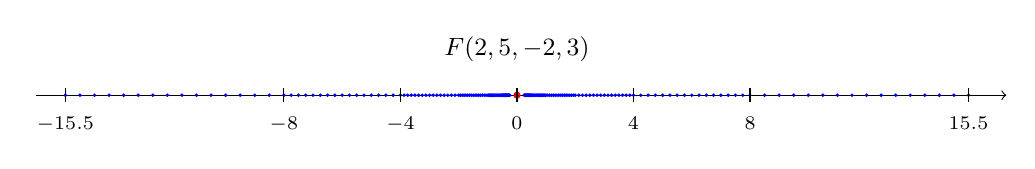
\begin{tikzpicture}[x=0.37cm,y=1cm]
  % Zahlengerade
  \draw[->] (-16.5,0) -- (16.8,0);

  % Alle positiven und negativen Maschinenzahlen
  \foreach \e in {-2,-1,0,1,2,3} {
    \foreach \j in {0,...,15} {
      \pgfmathsetmacro{\x}{2^(\e)*(1+\j/16)}
      \fill[blue] (\x,0) circle (0.7pt);
      \fill[blue] (-\x,0) circle (0.7pt);
    }
  }

  % Null
  \fill[red] (0,0) circle (1.3pt);

  % Beschriftung
  \foreach \x in {-15.5,-8,-4,0,4,8,15.5} {
    \draw (\x,0.09) -- (\x,-0.09);
    \node[below,font=\scriptsize] at (\x,-0.15)
      {$\x$};
  }

  \node[above,font=\small] at (0,0.3)
    {$F(2,5,-2,3)$};
\end{tikzpicture}
\end{center}

\nt{
  Die Maschinenzahlen sind nicht gleichmäßig
  auf der Zahlengeraden verteilt.

  Je größer der Exponent $E$, desto größer
  ist der Abstand zwischen benachbarten
  Maschinenzahlen.

  Die Schrittweite beträgt
  \[
    \Delta_E=2^{E-4}.
  \]
}


\subsection*{e) Maximaler Rundungsfehler}

\begin{myproof}
  Wir untersuchen zunächst den absoluten
  und anschließend den relativen Rundungsfehler.

  \medskip
  \textbf{1. Maximaler absoluter Rundungsfehler:}

  Zwei benachbarte positive Maschinenzahlen
  mit demselben Exponenten $E$ haben die Form
  \begin{align*}
    a&=2^E\left(1+\frac j{16}\right),\\
    b&=2^E\left(1+\frac{j+1}{16}\right).
  \end{align*}

  Ihr Abstand ist
  \begin{align*}
    b-a
    &=2^E\left(
      \frac{j+1}{16}-\frac j{16}
    \right)\\
    &=2^{E-4}.
  \end{align*}

  Da auf die nächstgelegene Maschinenzahl
  gerundet wird, beträgt der maximale
  absolute Fehler die Hälfte dieser Schrittweite:
  \[
    |x-\operatorname{rd}(x)|
    \le\frac12\cdot2^{E-4}
    =2^{E-5}.
  \]

  Der größte zulässige Exponent ist $E=3$.
  Somit gilt
  \[
    |x-\operatorname{rd}(x)|
    \le2^{3-5}
    =\frac14.
  \]

  Diese Schranke wird beispielsweise für
  $x=8{,}25$ erreicht, da die beiden
  benachbarten Maschinenzahlen $8$ und
  $8{,}5$ sind.

  Also beträgt der maximale absolute
  Rundungsfehler
  \[
    \boxed{\Delta_{\max}=\frac14=0{,}25.}
  \]

  \medskip
  \textbf{2. Maximaler relativer Rundungsfehler:}

  Der relative Rundungsfehler ist definiert durch
  \[
    \varepsilon
    :=\frac{|x-\operatorname{rd}(x)|}{|x|}.
  \]

  Wegen der Symmetrie des Maschinenzahlbereichs
  genügt es, positive Zahlen zu betrachten.

  Seien $a$ und $a+\Delta_E$ zwei benachbarte
  positive Maschinenzahlen, wobei
  \[
    \Delta_E=2^{E-4}.
  \]

  Der größte relative Fehler innerhalb dieses
  Intervalls tritt am Mittelpunkt auf:
  \[
    x=a+\frac{\Delta_E}{2}.
  \]

  Dort gilt
  \[
    |x-\operatorname{rd}(x)|
    =\frac{\Delta_E}{2}.
  \]

  Somit erhalten wir
  \[
    \varepsilon
    \le
    \frac{\Delta_E/2}
         {a+\Delta_E/2}.
  \]

  Da $a\ge2^E$, folgt
  \begin{align*}
    \varepsilon
    &\le
      \frac{2^{E-5}}
           {2^E+2^{E-5}}\\
    &=\frac{1}{2^5+1}\\
    &=\frac1{33}.
  \end{align*}

  Diese Schranke ist scharf, da sie
  beispielsweise für den Mittelpunkt zwischen
  den Maschinenzahlen
  \[
    2^{-2}
    \quad\text{und}\quad
    2^{-2}+2^{-6}
  \]
  erreicht wird.

  Somit beträgt der maximale relative
  Rundungsfehler
  \[
    \boxed{
      \varepsilon_{\max}
      =\frac1{33}
      \approx0{,}0303.
    }
  \]

  Dies entspricht ungefähr $3{,}03\,\%$.
\end{myproof}

\newpage
\section*{Aufgabe 5}

\qs{}{
  Implementieren Sie eine Klasse
  \texttt{BigInt}, die das Rechnen mit
  beliebig großen natürlichen Zahlen
  erlaubt.

  Nutzen Sie zum Abspeichern der Dezimalstellen
  einer Zahl den Datentyp
  \texttt{std::vector}.

  Implementieren Sie analog zur Klasse
  \texttt{Fraction} eine Funktion
  \texttt{add} zur Addition zweier
  \texttt{BigInt}-Objekte sowie eine
  Möglichkeit zur Ausgabe eines
  \texttt{BigInt}-Objekts.
}

\sol
\codefile{rust.h}{C++}
\codefile{bigint.h}{C++}
\codefile{main.cpp}{C++}
\end{document}
